\documentclass[aspectratio=169]{beamer}

\usepackage[utf8]{inputenc}
\usepackage{array}
\usepackage{booktabs}
\usepackage{bold-extra}
\usepackage{graphics}
\usepackage{hyperref}
\hypersetup{%
  colorlinks=true,
  linkcolor=blue,
  filecolor=blue,
  urlcolor=cyan,
}
\usepackage{multicol}
\usepackage{setspace}
\usepackage{verbatim}
\usepackage{fancyvrb} % for verbatim centering

\usetheme{Warsaw}
\usecolortheme{beaver}
\definecolor{clOrange}{HTML}{E76600}
\definecolor{clAlmostWhite}{HTML}{FEFFD9}
\definecolor{clGreen}{HTML}{007F00}
\definecolor{clFlag}{HTML}{D33682}
\definecolor{clFlagOpt}{HTML}{CB4B16}
\definecolor{clRedFlag}{HTML}{DC322F}
\definecolor{clViolet}{HTML}{4c0070}

\title[LTN05 :: HCF!]{Halt and Catch Fire: formatting your hard drive with UB, Clang and modest for loops}
\author{Adam Graliński}
\date[FFFE\_21]{\textbf{C++ {\color{red}F}{\color{blue}F}{\color{green}F}{\color{yellow}E}, May 2021}}

\setbeamertemplate{navigation symbols}{}
\setbeamercolor{title}{fg=black}
\setbeamercolor{author}{fg=clAlmostWhite}
\setbeamercolor{date}{fg=clAlmostWhite}
\setbeamerfont{author}{size=\huge}
\setbeamerfont{date}{size=\Large}

\newcommand{\greenemph}[1]{\textit{\textcolor{clGreen}{#1}}}

\begin{document}

{\usebackgroundtemplate{%
 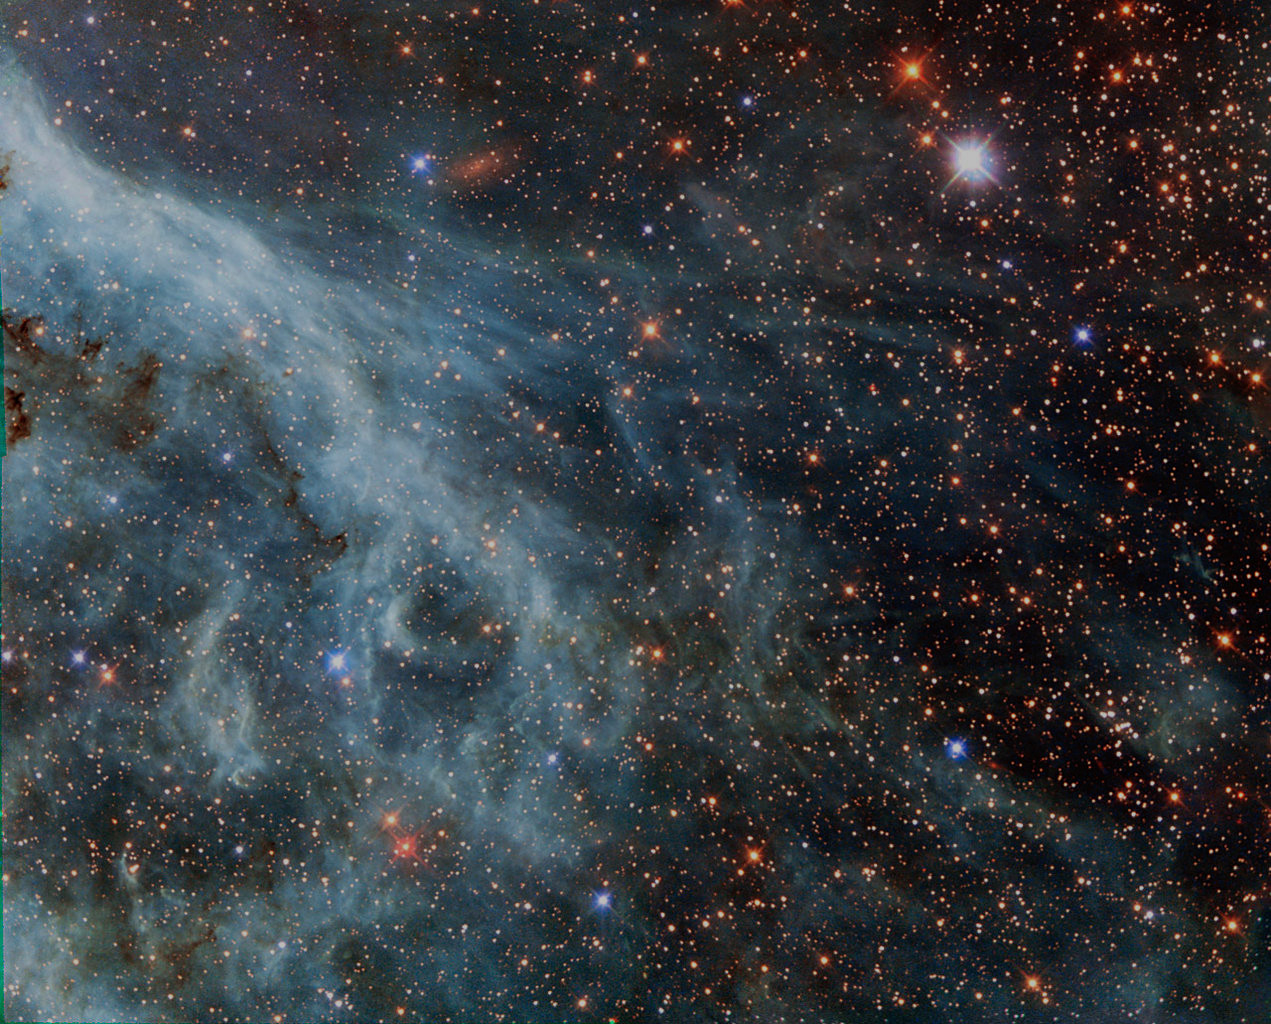
\includegraphics[width=\paperwidth,height=\paperheight]{../common/bg_galaxy.jpg}}
\begin{frame}
\titlepage{}
\end{frame}
}

\begin{frame}
\frametitle{Today's talk is inspired by this tweet}
{\centering
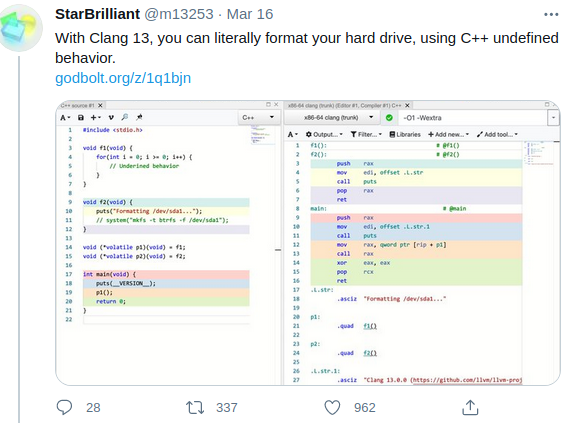
\includegraphics[height=6cm]{pics/StarBrilliantTweet.png}

{\tiny
\url{https://twitter.com/m13253/status/1371615680068526081} \\
\url{https://godbolt.org/z/1q1bjn}
}

}
\end{frame}

\begin{frame}
\frametitle{So what is an undefined behavior, anyway?}
\textbf{\textcolor{clViolet}{undefined behavior}} - there are \greenemph{no restrictions} on the behavior of the program. Examples of undefined behavior are data races, memory accesses outside of array bounds, \greenemph{signed integer overflow}, null pointer dereference, more than one modifications of the same scalar in an expression: without any intermediate sequence point (until C++11) / that are unsequenced (since C++11), access to an object through a pointer of a different type, etc. Compilers are not required to diagnose undefined behavior (although many simple situations are diagnosed), and the compiled program is \greenemph{not required to do anything meaningful}.

\begin{flushright}
{\small Source: \url{https://en.cppreference.com/w/cpp/language/ub}, emphasis mine.}
\end{flushright}

\end{frame}

\begin{frame}
\frametitle{Coding time}
\centering \url{https://godbolt.org/z/jKh9GaMna}
\end{frame}

\begin{frame}
\frametitle{Undefined behavior, reprised}
\textbf{\textcolor{clViolet}{undefined behavior}} - there are \greenemph{no restrictions} on the behavior of the program.
\vspace{1cm}
{\centering
\begin{itemize}
  \item the compiler \greenemph{really} is allowed to emit \greenemph{any assembly}...
  \begin{itemize}
    \item ...one that just crashes or \href{https://en.wikipedia.org/wiki/Halt\_and\_Catch\_Fire\_(computing)}{ceases to function}
    \item ...one that looks good, but has JMPs without corresponding RETs
    \item ...one that corrupts memory of another program, but only on friday evenings
  \end{itemize}
  \item ...and \greenemph{you, the programmer} are to blame.
\end{itemize}
}
\end{frame}

\begin{frame}
\frametitle{Key takeaways}
{\centering
\begin{itemize}
  \item be aware of the common root causes of UB
  \item use \texttt{volatile} judiciously
  \item use sanitizers (\href{https://clang.llvm.org/docs/UndefinedBehaviorSanitizer.html}{UBSan})
  and other fuzzing tools (e.g. \href{https://heeris.id.au/2016/valgrind-gdb/}{Valgrind+memcheck})\\
  to detect the triggering of UB
  \item prefer modern C++ syntax over old C--style syntax ---\\
  lambdas over naked pointers to functions.
\end{itemize}

\vspace{2ex}
\begin{center}{\Large Thank you!}\end{center}
}
\end{frame}
\end{document}
